\section{行程詳細}
\vspace{1em}
\subsection*{東北・北海道新幹線}
\addcontentsline{toc}{subsection}{東北・北海道新幹線}
\begin{table}[htb]
	\centering
	%\begin{tabular}{Wc{2cm}Wr{3.5cm}Wr{3.5cm}}
	\begin{tabular}{crr}
		\toprule
		&  \multicolumn{1}{c}{\textbf{行き}} &  \multicolumn{1}{c}{\textbf{帰り}}\\
		\midrule
		\rowcolor{lightgray!20}
		\multicolumn{1}{c|}{\textbf{日時}}     & 2月9日(日) & 2月11日(火)\\ 
		\multicolumn{1}{c|}{\textbf{列車名}} & はやぶさ17号 & はやぶさ110号\\
		\rowcolor{lightgray!20}
		\multicolumn{1}{c|}{\textbf{出発}} & 東京 10:18 & 仙台 11:52 \\
		\multicolumn{1}{c|}{\textbf{到着}} & 仙台 17:22 & 東京 18:56\\
		\rowcolor{lightgray!20}
		\multicolumn{1}{c|}{\textbf{席1}} & 3号車17番D席 & 3号車2番E席\\ 
		\multicolumn{1}{c|}{\textbf{席2}} & 3号車17番E席 & 3号車2番D席\\
		\bottomrule
	\end{tabular}
\end{table}

\begin{figure}[H]
	\centering
	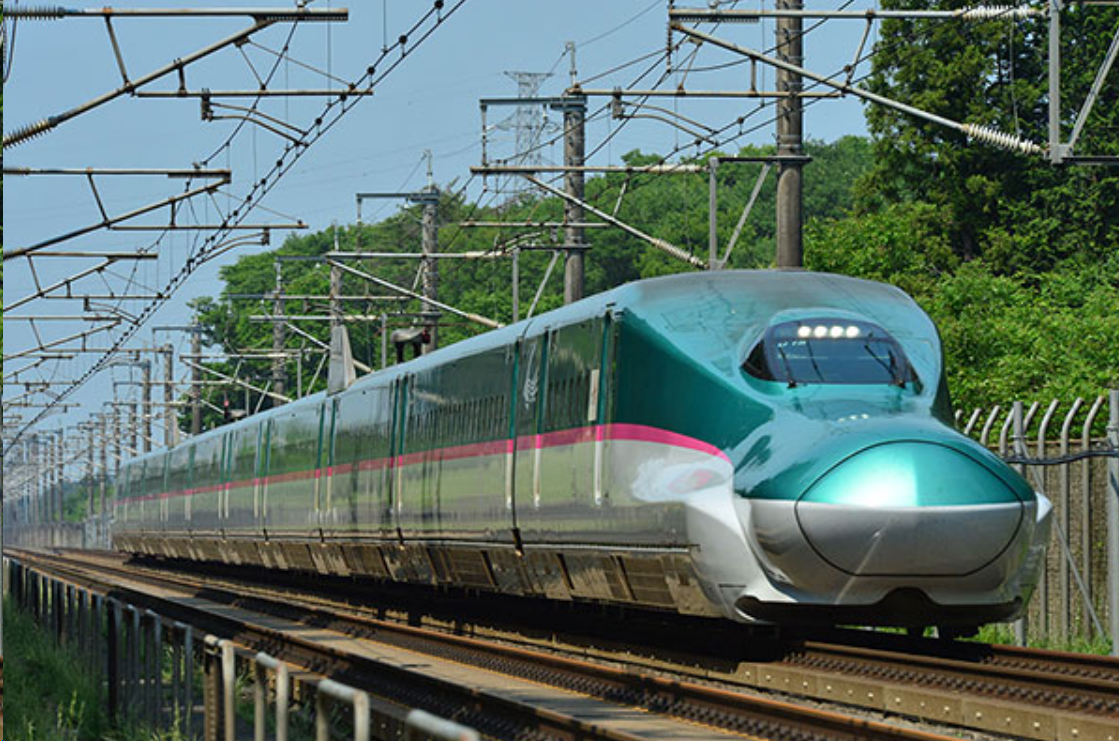
\includegraphics[width=0.7\linewidth]{img/hayabusa}
	\caption{E5系東北・北海道新幹線はやぶさ}
	\label{fig:hayabusa}
\end{figure}
